\section{Effective laws after eliminating variables}
\label{section:loss-dynamics-and-the-choice-of-scale}

To decide which distinctions are worth retaining, we also need to say what counts as an error. A loss function says which answers we prefer. It does not yet say how a system moves between them. The distinction matters because two procedures can have the same optimum and radically different routes towards it. A probability distribution over possible configurations gives one way to describe both uncertainty and exploration. Relative entropy then prices departure from a reference distribution, while a generator specifies the actual motion.

The Law of Laws develops this combination in the functional
\begin{equation}
 {\cal F}[p]=\sum_x p(x)K(x)+M\sum_x p(x)\log\frac{p(x)}{q(x)},
 \qquad
 p_*(x)=\frac{q(x)e^{-K(x)/M}}{Z}.
 \label{eq:law-functional}
\end{equation}
Here $p$ is a normalised distribution, $q$ a positive normalised reference, $K$ the cost of a configuration and $M>0$ the price of concentrating probability away from $q$. The normalising constant is $Z=\sum_xq(x)e^{-K(x)/M}$. Substitution gives the exact identity
\[
 {\cal F}[p]-{\cal F}[p_*]=M D_{\rm KL}(p\Vert p_*),
 \qquad {\cal F}[p_*]=-M\log Z.
\]
The preferred distribution is therefore fixed by an explicit competition between cost and concentration.~\cite{Reference0e02fc} The relative entropy on the right measures the excess objective.

This construction survives elimination of hidden variables in a useful sense. Write the configuration as $(y,\xi)$, with retained coordinate $y$ and discarded coordinate $\xi$. Summing over $\xi$ gives the effective cost
\begin{equation}
 K_{\rm eff}(y)
 =-M\log\sum_\xi q(\xi|y)e^{-K(y,\xi)/M}.
 \label{eq:effective-law}
\end{equation}
The marginal distribution has the same form as Eq.~\eqref{eq:law-functional}, now with reference $q(y)$ and cost $K_{\rm eff}(y)$. A description can remain in one mathematical family while its parameters change with resolution. For the source's elementary Ising example, each spin is a sign $\sigma_i=\pm1$ and a neighbouring pair has energy $-J\sigma_i\sigma_{i+1}$. Eliminating a middle spin means summing its two possible signs. For retained neighbours $a,c=\pm1$, the factor is $\sum_{u=\pm1}e^{Ju(a+c)/M}=2\cosh[J(a+c)/M]$. Matching the factors for $a=c$ and $a=-c$ changes the nearest-neighbour coupling to $J'=(M/2)\log\cosh(2J/M)$. The coordinate $x=\tanh(J/M)$ obeys the simple map $x'=x^2$. This is a concrete instance of the renormalisation idea: follow how an effective description changes, rather than insisting that its original parameters survive intact.

A stationary distribution does not specify a clock. Different generators can preserve the same distribution, and non-reversible ones can circulate probability around it. The equilibrium elimination in Eq.~\eqref{eq:effective-law} consequently does not establish the dynamical closure in Eq.~\eqref{eq:closure-residual}. The two results complement one another. One constructs an effective cost. The other tests whether the chosen retained state has enough information to evolve autonomously.

\subsection{A subsystem retains its surroundings' influence}
Eliminating variables becomes a physical question when they describe an interacting environment. A qubit in a device is not an isolated two-state object. It interacts with nearby modes, control circuitry and other degrees of freedom. Those interactions can change both its equilibrium probabilities and the information needed to predict its motion. Drawing a boundary around the qubit does not switch the interactions off. It changes what we must encode on the inside if we no longer describe the outside explicitly. A qubit has two basis states. We write a state column vector as $|\psi\rangle$ and its conjugate transpose as $\langle\psi|$, so $\langle\psi|O|\psi\rangle$ is ordinary matrix multiplication giving the mean measured value of an observable $O$. Observables are represented by Hermitian matrices, equal to their conjugate transpose and with real eigenvalues. The energy observable is called the Hamiltonian.

Let $S$ denote the subsystem and $B$ its surroundings, conventionally called a bath. Their joint state space is the tensor product $\mathcal H_S\otimes\mathcal H_B$: a joint basis labels one system state and one bath state. The full Hamiltonian is
\begin{equation}
 H_{SB}=H_S\otimes I_B+I_S\otimes H_B+V,
 \qquad
 \rho_{SB}^{\rm eq}=\frac{e^{-\beta H_{SB}}}{Z_{SB}},
 \qquad
 Z_{SB}=\operatorname{Tr}_{SB}e^{-\beta H_{SB}}.
 \label{eq:open-composite}
\end{equation}
$H_S$ and $H_B$ are the uncoupled energy operators, $V$ is their interaction and $I$ is the identity on the indicated space. Here $\beta=1/(k_{\rm B}T_{\rm phys})$ is physical inverse temperature, with Boltzmann's constant $k_{\rm B}$. Assume $T_{\rm phys}>0$ and finite partition functions. The exponential weights joint energy eigenstates by their thermal probabilities. The density matrix $\rho_{SB}$ is a positive matrix of unit trace: its diagonal entries are probabilities in the chosen basis, while its off-diagonal entries encode phase coherence. The trace $\operatorname{Tr}$ sums diagonal entries.

The reduced state is $\rho_S=\operatorname{Tr}_B\rho_{SB}$. This \emph{partial trace} sums over an orthonormal bath basis while leaving a matrix on the system:
\begin{equation}
 (\rho_S)_{ij}=\sum_\mu
 \langle i,\mu|\rho_{SB}|j,\mu\rangle,
 \qquad
 \operatorname{Tr}_S(A\rho_S)
 =\operatorname{Tr}_{SB}[(A\otimes I_B)\rho_{SB}].
 \label{eq:partial-trace}
\end{equation}
The second identity explains why this is the right retained object: it reproduces every observable $A$ measured on $S$ alone. It does not retain every system--bath correlation. Distinct joint states can therefore have the same reduced state.

At equilibrium, the environmental influence can be kept in an effective energy operator. Define the uncoupled bath partition function $Z_B=\operatorname{Tr}_B e^{-\beta H_B}$ and
\begin{equation}
 R_S=\operatorname{Tr}_B e^{-\beta H_{SB}},
 \qquad
 H_{\rm MF}(\beta)=-\frac1\beta\log\frac{R_S}{Z_B},
 \qquad
 \rho_S^{\rm eq}=\frac{e^{-\beta H_{\rm MF}}}{Z_{\rm MF}},
 \quad Z_{\rm MF}=\frac{Z_{SB}}{Z_B}.
 \label{eq:mean-force-normalised}
\end{equation}
This is the \emph{Hamiltonian of mean force}. The logarithm acts on the positive reduced operator. Dividing by $Z_B$ fixes its scalar energy convention, while dividing by $Z_{\rm MF}$ normalises the system state. These are different operations: $R_S/Z_B$ is generally not a unit-trace density matrix. If $V=0$, the exponential factorises, the bath trace contributes $Z_B$, and $H_{\rm MF}=H_S$. With interaction, $H_{\rm MF}$ can depend on temperature and need not have the same eigenvectors or energy spacings as $H_S$. This is the operator counterpart of eliminating $\xi$ in Eq.~\eqref{eq:effective-law}.~\cite{McCaulded509}

A small commuting example makes the change physical without requiring a bath approximation. Take two spins labelled $q,u=\pm1$, with joint energy $\epsilon q/2+\omega u/2+gqu$. The first spin is retained, the second is summed out. Its two possible surroundings contribute
\[
 R_S(q)=e^{-\beta\epsilon q/2}\,2\cosh[\beta(\omega/2+gq)],
 \qquad
 H_{\rm MF}(q)=\frac{\epsilon q}{2}
 -\frac1\beta\log\frac{\cosh[\beta(\omega/2+gq)]}{\cosh(\beta\omega/2)}.
\]
Here $\epsilon$ and $\omega$ set the uncoupled spin splittings and $g$ the interaction energy. Their units are energy. The effective splitting of the retained spin is
\[
 H_{\rm MF}(+1)-H_{\rm MF}(-1)
 =\epsilon-\frac1\beta\log
 \frac{\cosh[\beta(\omega/2+g)]}{\cosh[\beta(\omega/2-g)]}.
\]
The preference of the surrounding spin has changed the retained spin's thermal odds. In the symmetric case $\omega=0$, the interaction instead contributes the same scalar shift to both states. Which correlations matter therefore depends on symmetry, temperature and the observable as well as coupling strength.

The same boundary has a dynamical consequence. The joint density matrix evolves by $i\hbar\dot\rho_{SB}=[H_{SB},\rho_{SB}]$, where $\hbar$ is the reduced Planck constant and $[A,B]=AB-BA$. Taking the partial trace gives
\begin{equation}
 i\hbar\dot\rho_S=[H_S,\rho_S]
       +\operatorname{Tr}_B[V,\rho_{SB}].
 \label{eq:open-dynamical-residual}
\end{equation}
The second term still depends on the joint state. Two preparations with the same $\rho_S$ but different correlations can have different subsequent motion, just as the same region mass had two different escape rates in the four-state example. One can retain more environmental coordinates, make a justified closure approximation, or eliminate them into a history-dependent term of the kind in Eq.~\eqref{eq:general-memory}. The mean-force operator reproduces equilibrium statistics. It is not, by that fact alone, the generator of the reduced real-time motion.

This is the open-systems version of the representational question. An adequate description carries the influence that crosses its chosen boundary, not necessarily all the surrounding detail. The papers \emph{Equilibrium from the Inside Out} and \emph{Dual Representatives of Mean-Force Equilibrium} pursue explicit ways of representing that influence.~\cite{McCaulbab685} The construction keeps the environmental influence in an object defined on the subsystem itself, making the choice of boundary part of the calculation.

\subsection{Absorb the difficult coupling before approximating}
The ground-state extension turns that representational choice into an analytical calculation. A spin strongly coupled to oscillators can be difficult to describe in the uncoupled basis because each spin orientation shifts the oscillators' preferred positions. Conditional displacement builds those shifts into the basis exactly. What remains is a bounded spin-flip operator. The bath spectrum then predicts the ground energy, the local spin state and its conditional surroundings, with independent diagonalisation of the original Hamiltonian providing the comparison in Fig.~\ref{fig:dd-hmf-physical-ground-state-20261016}.~\cite{McCaul2026e37796}

Consider the unbiased spin--boson Hamiltonian, in units with $\hbar=1$,
\begin{equation}
 H=H_B+g\tau_z B-\frac{\Delta}{2}\tau_x,
 \qquad H_B=\sum_k\nu_k b_k^\dagger b_k,
 \qquad B=\sum_kv_k(b_k+b_k^\dagger).
 \label{eq:hmf-physical-model}
\end{equation}
The two eigenvalues of $\tau_z$ label the spin orientations that exert opposite forces on the bath. The matrix $\tau_x$ flips them, with tunnelling energy $\Delta>0$. The operators $b_k^\dagger$ and $b_k$ add and remove one excitation of oscillator $k$, whose excitation energy is $\nu_k>0$. The real coefficient $v_k$ has units of energy and $g$ is a dimensionless coupling strength. We keep finitely many modes with gap $\nu_{\min}=\min_k\nu_k>0$ and expand in $\Delta<\nu_{\min}$, not in $g$.

Completing the oscillator squares shifts each mode by $d_k=gv_k/\nu_k$ and lowers the common energy by $g^2\lambda_0$, where $\lambda_0=\sum_kv_k^2/\nu_k$. The displacement operator is
$D(d)=\exp[\sum_kd_k(b_k^\dagger-b_k)]$. It changes coordinates without discarding the displaced bath states. Let $P_B=(-1)^{\sum_k b_k^\dagger b_k}$ distinguish even from odd total excitation number. In a sector of conserved combined spin and bath parity $\kappa=\pm1$, the joint eigenproblem becomes
\begin{equation}
 H_\kappa=H_B-g^2\lambda_0-\frac{\kappa\Delta}{2}T_g,
 \qquad T_g=D(2d)P_B,
 \qquad T_g^\dagger=T_g,\quad T_g^2=I.
 \label{eq:hmf-bounded-tunnelling}
\end{equation}
The last identity is the useful change: $\|T_g\|=1$ for every $g$. An interaction that was unbounded in oscillator coordinates has been absorbed into the representation, leaving a correction of size $\Delta/2$.

A spin flip exchanges the two displaced oscillator configurations. Let $|0\rangle$ be the oscillator vacuum. The correlation is the matrix element $C_g(t)=\langle0|T_g e^{-tH_B}T_g|0\rangle$, with imaginary time $t$ measured in inverse energy. For the specified bath it is
\begin{equation}
 C_g(t)=
 \exp\!\left[-4g^2\sum_k\frac{v_k^2}{\nu_k^2}
                 (1-e^{-\nu_k t})\right],
 \qquad
 S_g=\exp\!\left[-2g^2\sum_k\frac{v_k^2}{\nu_k^2}\right].
 \label{eq:hmf-retained-spectrum}
\end{equation}
$S_g$ is the overlap of the two displaced vacua. $C_g(t)$ retains the distribution of excitation energies deposited by a flip, rather than only their total energy shift. Define its excited-state inverse moments
\[
 A_g=\int_0^\infty[C_g(t)-S_g^2]\,dt,
 \qquad
 B_g=\int_0^\infty t[C_g(t)-S_g^2]\,dt.
\]
Subtracting $S_g^2$ removes the zero-excitation contribution. In an eigenbasis $H_B|n\rangle=E_n|n\rangle$, the excited terms of the correlation are $|\langle n|T_g|0\rangle|^2e^{-tE_n}$. Integrating therefore gives $A_g=\sum_{n\ne0}|\langle n|T_g|0\rangle|^2/E_n$ and $B_g=\sum_{n\ne0}|\langle n|T_g|0\rangle|^2/E_n^2$. These are the virtual-excitation denominators in the perturbative expansion. On the positive-parity ground branch,
\begin{equation}
 E_0=-g^2\lambda_0-\frac{\Delta S_g}{2}
                      -\frac{\Delta^2 A_g}{4}+O(\Delta^3),
 \qquad
 \langle\tau_x\rangle_0=S_g+\Delta A_g+O(\Delta^2),
 \quad \langle\tau_z\rangle_0=0.
 \label{eq:hmf-ground-prediction}
\end{equation}
The first spin contribution comes from the overlap of the displaced vacua. The next comes from excursions through the excited bath. The spin expectation follows from the energy by the Hellmann--Feynman identity $\langle\tau_x\rangle_0=-2\partial_\Delta E_0$. Both are calculated from the spectrum, without fitting the ground-state data. The fixed gap and bounded perturbation also give an explicit remainder for the displayed energy approximation $E_0^{(2)}$: for $\Delta<\varrho<\nu_{\min}$,
\[
 |E_0-E_0^{(2)}|
 \le \frac{\varrho}{2}
       \frac{(\Delta/\varrho)^3}{1-\Delta/\varrho}.
\]
Thus the change of representation makes the approximation controllable even when the physical bath coupling is not small.

The construction retains more than a local spin average. Write $Q_B=I-|0\rangle\langle0|$ for removal of the oscillator vacuum and
$|\eta_g\rangle=Q_BH_B^{-1}Q_BT_g|0\rangle$. The normalised bath trial state
$|\psi_{\rm tr}\rangle=(|0\rangle+\Delta|\eta_g\rangle/2)/\sqrt{1+\Delta^2B_g/4}$
reconstructs the physical joint state as
\begin{equation}
 |\Psi_{\rm tr}\rangle=
 \frac{|+\rangle D(-d)|\psi_{\rm tr}\rangle
       +|-\rangle D(d)P_B|\psi_{\rm tr}\rangle}{\sqrt2}.
 \label{eq:hmf-conditional-bath}
\end{equation}
Here $|\pm\rangle$ are the two $\tau_z$ orientations. This state can answer questions about the conditional bath as well as the spin, and its energy is a variational upper bound. The source comparison checks the joint vector separately from the reduced state.

\begin{figure}[htbp]
\centering
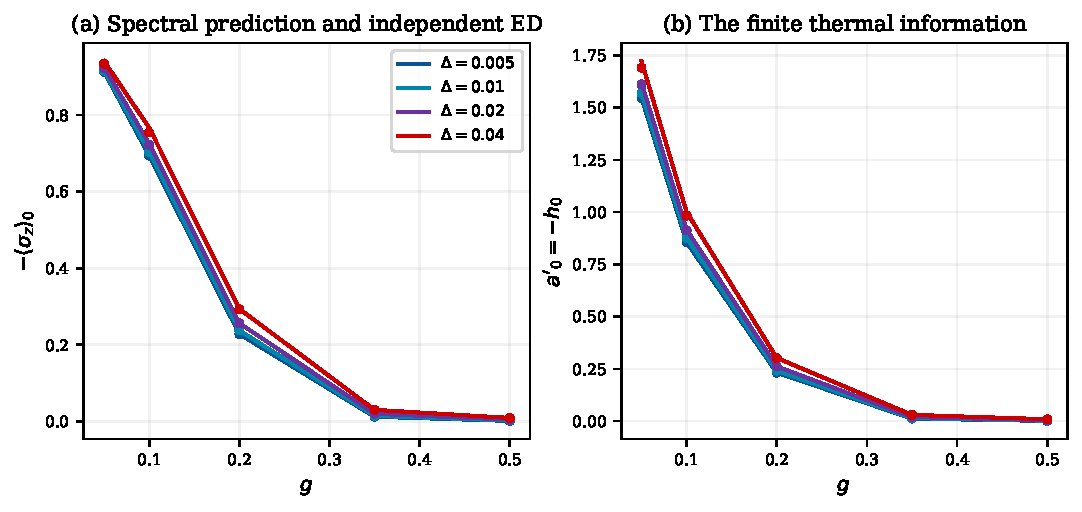
\includegraphics[width=\linewidth]{../figures/generated/dd-hmf-physical-ground-state-20261016.pdf}
\caption{The bath spectrum predicts the cold spin before numerical comparison.~\cite{McCaul2026e37796} (a) Lines show $-\langle\sigma_z\rangle_0=S_g+\Delta A_g$ and points show independent diagonalisation of the original Hamiltonian, with $\sigma_z=-\tau_x$. (b) The normalised conditional-bath trial predicts the dimensionless thermal coordinate $a'_0=-h_0$, compared with the coordinate obtained from those numerical ground states. Here $h_0=-\operatorname{arctanh}r_0$, where $r_0$ is the reduced spin's Bloch-vector length. The two bath energies are $\nu_k=(0.2,1.8)$ and $v_k^2=4\nu_k e^{-\nu_k/2}$ in the chosen energy unit. The legend gives the tunnelling energy $\Delta$ and the horizontal axis the coupling $g$. Bath coupling is retained exactly, while tunnelling is controlled relative to the fixed bath gap. The comparison includes two oscillator cutoffs and a separate joint-vector check.}
\label{fig:dd-hmf-physical-ground-state-20261016}
\end{figure}

\subsection{Carry the answer back}
In the original energy axes, $\sigma_z=-\tau_x$. With $r_0=S_g+\Delta A_g+O(\Delta^2)$, the reduced ground state is $\rho_0=(I-r_0\sigma_z)/2$. Its eigenvalues $(1\pm r_0)/2$ specify the local probabilities and entropy. More generally, the three spin averages form the Bloch vector $\mathbf m$ in $\rho=(I+\mathbf m\cdot\boldsymbol\sigma)/2$, where $\boldsymbol\sigma$ denotes the three Pauli spin matrices. Cooling the composite therefore need not make the subsystem pure: its entanglement with the displaced bath survives. The dimensionless coordinate $h_0=-\operatorname{arctanh}r_0$ records the corresponding population imbalance. The dual-reference construction carries this predicted state to a finite reference coordinate $a'_0=-h_0$. Here $a'=\beta'\omega'_r/2$ is half the chosen reference splitting $\omega'_r$ in units of its temperature. The endpoint is shown in Fig.~\ref{fig:dd-hmf-physical-ground-state-20261016}(b).

A reference change must preserve more than the appearance of a normalised matrix. Let $\mathcal R=R_S/Z_B$ be the unnormalised mean-force operator from Eq.~\eqref{eq:mean-force-normalised}. Factor it as $\mathcal R=G_b\Xi_bG_b$, where $G_b$ is a strictly positive reference thermal factor and $\Xi_b$ the remaining influence. For another strictly positive factor $G_r$, define
\begin{equation}
 A=G_r^{-1}G_b,\qquad
 \Xi_r=A\Xi_bA^\dagger,\qquad
 G_r\Xi_rG_r=\mathcal R,\qquad
 \langle O\rangle=
 \frac{\operatorname{Tr}(\Xi_rG_rOG_r)}
      {\operatorname{Tr}(\Xi_rG_r^2)}.
 \label{eq:hmf-reference-transport}
\end{equation}
At finite temperature this identity retains the full operator. In taking its cold limit, the scalar ground-energy factor $e^{-\beta E_0}/Z_B$ accompanies the limiting reduced state. The denominator retains the partition weight, the numerator the measured observable $O$. Their order matters when the factors do not commute. A convenient reference for a predicted state with Bloch vector $\mathbf m_0$ points along $\mathbf n_r=-\mathbf m_0/|\mathbf m_0|$. The state is diagonal along this adapted axis, while the axis itself retains its physical orientation. In the mixed case $0<|\mathbf m_0|<1$, its finite coordinate is again $a'_{r,0}=\operatorname{arctanh}|\mathbf m_0|$. This transports the answer already calculated from the bath, including its scalar weight and observable interpretation.~\cite{McCaul2026e37796}

This suggests a concrete route to better machine-learning calculations. When a difficult interaction is already understood, represent it explicitly before asking an optimiser to learn or correct everything else. The remaining operator should expose a bounded correction, a useful spectrum or a measurable residual. The loss-operator diagnostics in the next section retain directions that a scalar objective hides. Gap-aware trial-space enlargement spends effort on omitted directions according to their effect on the answer. Task-directed memory retains the relations needed to reconstruct a query. The spin--bath calculation supplies a physical example of the same strategy with an analytic error control. Transferring it to a learning problem means identifying that problem's solvable structure, pricing the transformation and checking the reconstructed predictions against a matched-cost baseline. It is a method for designing and testing improved calculations, rather than a speed-up inferred merely from using quantum notation.

\subsection{When refinement changes the questions}
The reference transformation above preserves the same physical state. Changing resolution poses a different problem: the resolved distinctions themselves may change. This is the second thread developed in The Law of Laws, where quantum-like structure can appear when successive descriptions lose information in a way that cannot be absorbed into a change of scalar costs. The preceding closure residual tells us that a retained state is missing part of its evolution. Now ask whether refining that description merely changes the values attached to its resolved modes, or also changes which directions count as distinct modes. The latter requires an operator account of the change.

Foundations develops this question in \emph{Transporting a spectral description}, within Chapter 3's discussion of where discarded information went.~\cite{Reference0e02fc} To compare neighbouring descriptions, first specify a common inner-product space of fixed dimension and how its coordinates are transported. Write $\mathsf K_s$ for a differentiable Hermitian effective operator at description parameter $s$, and $\mathsf J_s$ for the anti-Hermitian generator of the chosen frame transport. Hermitian means equal to its conjugate transpose, while anti-Hermitian means its negative. The transport preserves inner products. We use different letters here from the probability generator $G$ and coarse map $C$: this is a smooth, fixed-rank comparison of the resolved operators.

An infinitesimal comparison map is $T_{s\to s+h}=I+h\mathsf J_s+o(h)$. The difference between transporting the old law and applying the new law is
\begin{equation}
 T_{s\to s+h}\mathsf K_s-\mathsf K_{s+h}T_{s\to s+h}
 =h\omega_s+o(h),\qquad
 \omega_s=[\mathsf J_s,\mathsf K_s]-\mathsf K'_s .
 \label{eq:refinement-residue-density}
\end{equation}
Here $[A,B]=AB-BA$, the prime denotes differentiation with respect to $s$, and $o(h)$ denotes terms smaller than first order as $h\to0$. The finite-step mismatch tends to zero as the step shrinks, but its density $\omega_s$ can remain nonzero. That is the quantity to follow through increasingly fine descriptions.

The distinction between diagonal and off-diagonal residue is the mechanism. Let $\lambda_i$ be a simple eigenvalue of $\mathsf K_s$ and $\Pi_i$ its spectral projector. Differentiating the eigenvalue equation gives
\begin{equation}
 \Pi_j\bigl(\Pi_i'-[\mathsf J_s,\Pi_i]\bigr)\Pi_i
 =-\frac{\Pi_j\omega_s\Pi_i}{\lambda_i-\lambda_j},
 \qquad j\ne i .
 \label{eq:refinement-projector-rotation}
\end{equation}
Diagonal residue shifts eigenvalues. Off-diagonal residue rotates the spectral directions after the chosen coordinate transport has been removed. A small gap allows a given mismatch to rotate those directions strongly. Merely adjusting a list of scalar penalties cannot describe that rotation.

For a fixed-coordinate example, choose $\mathsf J_s=0$ and a resolved direction $u_s=(\cos\nu s,\sin\nu s)^T$, with projector $\Pi_s=u_su_s^T$ and fixed nonzero rotation rate $\nu$. At $s=0$,
\[
 \lim_{h\to0}\frac{[\Pi_0,\Pi_h]}h
 =\nu\begin{pmatrix}0&1\\-1&0\end{pmatrix}.
\]
The projectors themselves become arbitrarily close as $h$ shrinks, yet in this fixed frame the rate at which their order matters stays finite. A co-rotating frame could remove this example's rotation. A residual claim therefore depends on which coordinate transport the comparison admits. Law of Laws~\cite{McCaulad9572} proposes a self-similar regime in which off-diagonal residue remains significant relative to the spectral gap. The effective description then keeps a noncommuting algebra of resolved distinctions instead of settling into one fixed spectral basis. This is the precise quantum-like feature that the refinement argument brings into the programme.

Foundations places that feature beside two further constructions. Chapter 2 tests whether overlapping measurement contexts admit one global assignment, while Chapter 3 exhibits classical averaging and reversible Markov examples with noncommuting operations or rotating eigenspaces. The distinction is productive: the spectral calculation identifies the persistent operator structure, and the context experiment asks which probability accounts it can support. This is an author-proposed connection. Connecting these constructions into a physical quantum reconstruction requires the specified event algebra, composition and measurement rule, as well as a calibrated action scale. These conditions specify the next reconstruction problem.

\subsection{Can the retained questions share one probability account?}
The four-state example asks whether a summary can carry a prediction forward in time. A different test is whether several summaries can be combined into one consistent account. Here the information at risk is which observations belong together. A \emph{context} is a set of measurements that can be made jointly. If an observable belongs to two contexts, its identity must remain the same in both. Foundations Chapter 2 asks whether the joint probability tables for overlapping contexts can all be obtained as marginals of one context-independent distribution.~\cite{McCaul85986c}

The two-qubit Peres--Mermin construction makes the obstruction elementary. In a two-state basis the Pauli matrices are
\[
 X=\begin{pmatrix}0&1\\1&0\end{pmatrix},\quad
 Y=\begin{pmatrix}0&-i\\i&0\end{pmatrix},\quad
 Z=\begin{pmatrix}1&0\\0&-1\end{pmatrix}.
\]
Here $i^2=-1$ and $I$ is the identity. For two qubits, $X\otimes I$ acts on the first and $I\otimes X$ on the second. Arrange the observables as
\[
 \begin{array}{ccc}
 X\otimes I&I\otimes X&X\otimes X\\
 I\otimes Z&Z\otimes I&Z\otimes Z\\
 X\otimes Z&Z\otimes X&Y\otimes Y
 \end{array}.
\]
Within each row or column the three matrices commute, so their joint outcome constraints can be tested.  Each has outcomes $+1$ or $-1$, and every row and column is a jointly measurable context. The operator products require
\[
 \begin{array}{c|ccc}
 \text{context}&1&2&3\\ \hline
 \text{row product}&+1&+1&+1\\
 \text{column product}&+1&+1&-1
 \end{array}.
\]
Suppose one value could be assigned to every cell independently of how it was measured. Multiplying all six context products would use each cell twice, giving $+1$. The required signs instead multiply to $-1$. At least one context constraint must fail. If $W$ counts agreement with each required sign as $+1$ and disagreement as $-1$, every such assignment and every probability mixture obeys $W\le4$, while the quantum product identities give $W=6$. The displayed operators specify the sign constraints without requiring a companion derivation. The crucial retained information is the overlap of measurement identities, not merely six unrelated summaries.

This is different from the dynamical closure residual: one tests a common probability account, the other tests autonomous evolution of a retained state. A change of coordinates or frame can change the matrices used to describe the same observables without changing their predictions. That freedom of representation must be distinguished from changing a measurement context, which changes the jointly accessible questions. The spectral-transport construction above makes one such frame comparison explicit. Together these connect retained distinctions, overlapping measurement contexts and changes of spectral frame.

\subsection{A loss with specified dynamics}
The changing spectral directions show why an operator can carry information that scalar costs alone miss. To use that idea in a calculation, we need a specified motion as well as a cost landscape. A stochastic dynamics supplies a concrete construction. Consider a coordinate moving down a smooth confining potential $V(x)$ while receiving random kicks:
\begin{equation}
 dX_t=-V'(X_t)\,dt+\sqrt{2T}\,dW_t,
 \qquad
 \partial_t p=\partial_x(V'p)+T\partial_x^2p.
 \label{eq:loss-diffusion}
\end{equation}
$W_t$ is standard Brownian motion and $T>0$ sets the noise intensity. Mobility has been set to one. With appropriate boundary conditions, the stationary density is $\pi(x)=Z^{-1}e^{-V(x)/T}$. Writing $p(x,t)=\sqrt{\pi(x)}\,\psi(x,t)$ transforms the evolution into
\begin{equation}
 T\partial_t\psi=-H_V\psi,\qquad
 H_V=-T^2\partial_x^2+\frac{(V')^2}{4}-\frac{T V''}{2}.
 \label{eq:loss-operator}
\end{equation}
This is a change of representation with a clear gain. The original density evolution becomes a self-adjoint spectral problem under the corresponding domain and boundary conditions. The weighted density norm $\int |p|^2/\pi\,dx$ becomes the ordinary squared norm of $\psi$. Relaxation modes can now be studied with operator methods.~\cite{Reference0e02fc}

The factor $T$ on the left is essential. For $V(x)=\kappa x^2/2$, the operator eigenvalues are $E_n=n\kappa T$, while the decay rates are $E_n/T=n\kappa$. Confusing the eigenvalues with rates would change the physical time scale. The stationary mode is $\psi_0=\sqrt{\pi}$ and has zero eigenvalue. This construction belongs to the established relationship between diffusion, factorised operators and supersymmetric quantum mechanics, developed mathematically in Witten's work.\footnote{E. Witten, \emph{Supersymmetry and Morse Theory}, Journal of Differential Geometry 17 (1982),661--692, \href{https://doi.org/10.4310/jdg/1214437492}{doi:10.4310/jdg/1214437492}.} Its role here is operational: a loss landscape and specified noise law supply an operator whose low modes describe relaxation.~\cite{Witten1982605ee8}

\subsection{Keep a useful correction visible}
The choice of objective can be just as consequential as the choice of dynamics. Suppose $n$ independently controlled two-level components should all end in their preferred state, and component $j$ succeeds with probability $p_j=\cos^2(\theta_j/2)$. Two losses have exactly the same perfect solution:
\begin{equation}
 C_G=1-\prod_{j=1}^n p_j,\qquad
 C_L=1-\frac{1}{n}\sum_{j=1}^n p_j.
 \label{eq:global-local-cost}
\end{equation}
The global loss rewards the complete conjunction. The local loss rewards each corrected component. For independently uniform angles, their derivative variances are
\begin{equation}
 {\rm Var}(\partial_j C_G)=\frac18\left(\frac38\right)^{n-1},
 \qquad
 {\rm Var}(\partial_j C_L)=\frac{1}{8n^2}.
 \label{eq:global-local-variance}
\end{equation}
A global demand can thus bury a useful local signal exponentially fast even when the answer itself is unchanged. Figure~\ref{fig:dd-global-local-feedback} makes the difference visible. Cerezo and colleagues use this example to distinguish cost-dependent concentration from the broader random-circuit barren-plateau mechanism established by McClean and colleagues.\footnote{M. Cerezo et al., \emph{Cost function dependent barren plateaus in shallow parametrized quantum circuits}, Nature Communications 12 (2021), \href{https://doi.org/10.1038/s41467-021-21728-w}{doi:10.1038/s41467-021-21728-w}. J. R. McClean et al., \emph{Barren plateaus in quantum neural network training landscapes}, Nature Communications 9 (2018), \href{https://doi.org/10.1038/s41467-018-07090-4}{doi:10.1038/s41467-018-07090-4}.} Locality is a design resource, not a guarantee that arbitrarily deep or poorly conditioned models train easily.~\cite{Cerezo2021232f10,McClean20183bd480}
\begin{figure}[htbp]
\centering
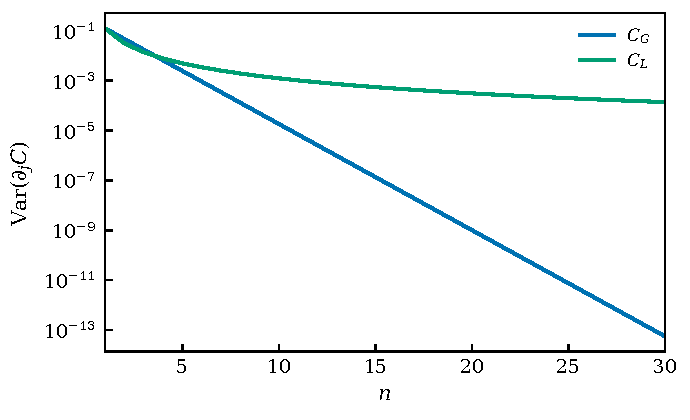
\includegraphics[width=\linewidth]{figures/portable-run-b69220b3a27348ad.result/dd-global-local-feedback.pdf}
\caption{The same optimum with different feedback. For the product-state example of Cerezo et al.~\cite{Cerezo2021232f10}, the global and local losses in Eq.~\eqref{eq:global-local-cost} have the same zero-cost target. With independent uniform angles, $\operatorname{Var}(\partial_j C_G)=\tfrac18(\tfrac38)^{n-1}$, while $\operatorname{Var}(\partial_j C_L)=1/(8n^2)$. Here $n$ is the number of qubits. Exact model variances isolate cost-dependent concentration.}
\label{fig:dd-global-local-feedback}
\end{figure}

\subsection{Combining local responses without instability}
Usable feedback needs more than a visible signal. Combining many responsive components can also make a correction too strong. Adaptive Normal Form and Phases of Hierarchy study this stability problem. In the latter's sampled model, a plant state $x_k$ relaxes towards $s\theta_k$ between updates,
\[
 x_{k+1}=r x_k+(1-r)s\theta_k,\qquad
 e_k=x_{k+1}-b\theta_k,\qquad
 \theta_{k+1}=\theta_k+\alpha R_N(e_k).
\]
Here $r=e^{-h/\tau_r}$ is the fraction of the previous state retained over sampling interval $h$, $\tau_r$ the relaxation time, $s$ the plant gain, $b$ the reference gain, and $\alpha$ the update size. The response of a noisy majority of $N$ components is approximated by
$R_N(e)\simeq{\rm erf}(\beta e\sqrt{N/2})$, so its small-signal slope is $G_N\simeq\beta\sqrt{2N/\pi}$. Increasing $N$ increases the loop gain $K=\alpha G_N$.

For $0<r<1$ and $b>s>0$, the linearised discrete dynamics is stable only when
\begin{equation}
 0<K<
 \frac{2(1+r)}{(1+r)b-(1-r)s}.
 \label{eq:feedback-bound}
\end{equation}
In the declared example, $\alpha=0.35$, $\beta=0.6$, $b=1.2$, $s=0.4$ and $r=e^{-1}$ put the Gaussian-response crossing near $N=138.25$. Adding responsive components can therefore destabilise a loop whose individual parts have not changed. The boundary quantifies the permitted response gain in this sampled loop.~\cite{McCaul630942}

The hierarchy in Phases of Hierarchy makes that change explicit. Let layer $\ell$ combine $n_\ell$ inputs, so $L$ aggregation layers represent $N=\prod_{\ell=1}^L n_\ell$ bottom-level components. In the paper's iterated Gaussian approximation, the expected response obeys $m_\ell(e)=\operatorname{erf}(\sqrt{n_\ell/2}\,m_{\ell-1}(e))$, with individual slope $m_0'(0)=\beta$. Differentiating each stage at zero and multiplying its slopes gives
\begin{equation}
 K_N^{(L)}=\alpha\beta\sqrt{\frac{2N}{\pi}}\,c^{L-1},
 \qquad c=\sqrt{\frac{2}{\pi}},
 \qquad
 N_c^{(L)}=N_c^{(1)}\left(\frac{\pi}{2}\right)^{L-1}.
 \label{eq:hierarchy-stability}
\end{equation}
Here $L=1$ is the flat aggregate. The factor $c$ is attenuation relative to a flat group of the same total size, not the absolute gain of each local block. One more aggregation layer therefore raises the population threshold by $\pi/2$ within this model. Figure~\ref{fig:dd-hierarchy-stability} shows the resulting phase diagram: a population of $200$ lies beyond the flat threshold but below the two-layer threshold at $\alpha=0.35$ and $h/\tau_r=1$. Slower updates provide another way to remain stable because the plant has longer to relax before the next correction.~\cite{McCaul630942}

Attenuating a response also has a cost. In the paper's separate depth-$L$ linear control cascade with attenuation $0<c<1$, the minimum squared-input effort needed to produce a unit apex response scales as $c^{-2(L-1)}$, once the control horizon is long enough to reach the apex. The cascade provides a separate measure of the intervention cost of attenuation. Adaptive Normal Form supplies a related gradient-feedback construction, but its effective gain contains two response derivatives and scales differently.~\cite{McCaul74663e} The common design question is where an aggregate response should be represented and acted upon, with its stability, signal and control costs accounted for.
\begin{figure}[htbp]
\centering
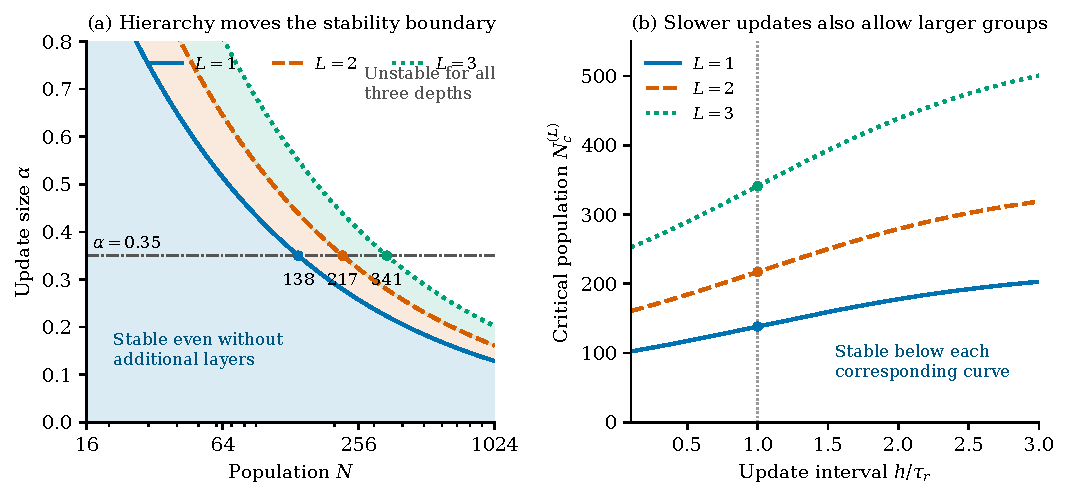
\includegraphics[width=\linewidth]{figures/hierarchy-run-d9f38e92caf64d82.result/dd-hierarchy-stability.pdf}
\caption{Hierarchy moves the stability boundary of the sampled feedback model. (a) At $h/\tau_r=1$, each curve separates stable dynamics below it from instability above it. The orange and green bands show additional parameter ranges stabilised by a second and third aggregation layer. The $\alpha=0.35$ slice crosses at $N_c^{(1)}=138.25$, $N_c^{(2)}=217.17$ and $N_c^{(3)}=341.13$. (b) At fixed $\alpha=0.35$, increasing the update interval also raises the critical population. In both panels $\beta=0.6$, $b=1.2$ and $s=0.4$. Curves use the iterated Gaussian expected-majority model of Phases of Hierarchy~\cite{McCaul630942}, not exact small-block voting or ANF's different feedback rule. The numerical checks of the linear boundary are retained with the figure's result record.}
\label{fig:dd-hierarchy-stability}
\end{figure}

These examples give representation a more demanding meaning than a relabelling of variables. A retained coordinate determines which history must be carried. A loss determines which corrections remain visible. A feedback architecture determines how many local responses can be combined without losing stability. The practical question is then whether these distinctions can guide a calculation that would otherwise be unnecessarily difficult.

